\section{Matrices usage example}

\vspace*{-0.2cm}


In this section, we present the service of an insurance company that manages insurance contracts to illustrate how the presented comparison matrices can be used in a real world scenario. This example is a light version of projects we have carried out at FABERNOVEL for former clients: large French insurance companies.

\subsection{Domain description}

To manage insurance contracts, the service holds five kinds of resources: (i) third-parties, (ii) contracts, (iii) warranties, (iv) cases and (v) services. Third-parties, for example customers or contractors, enter into contracts with the company. These contracts include warranties from the closed list that the company offers. For example a Person A has the following warranties: (i) damage coverage with a deductible of \$500 and a maximum repair amount of \$30.000 and (ii) premium vehicle loan in the event of immobilization of the damaged vehicle. A contract can have several cases. When an customer of the insurance has a claim the company creates a case that holds its details and the services provided to the insured. For example, Person A has a car accident, he opens the insurance's web application and reports a claim, which leads to the company opening a case. His car has been destroyed and he is expected to attend a diner. Thus, on the app, he asks for the loan of a car that he will immediately recover.

\subsection{Technological constraints}

The service has to communicate with both internal and external components. Internal components are front-end applications, such as mobile or web applications, and other kernel services, such as payments. External components are contractors APIs, for example taxi or mechanics companies.

In the insurance domain, there is a huge amount of business rules that determine (i) the warranties an insured can include in a contract and (ii) the available services for a case, based on the specificity of the given case and the warranties of the contract. Writing and maintaining these rules both on the server and its clients is very costly and error prone. Thus, we decided to keep these business rules on the server-side only. This constraint leads to the use of HATEOAS.

The project constitutes the core of the company's business, it should then be designed to meet future evolution of the company's IS. 
The service should therefore be Linked Data compatible. This enables the automatic creation of mash-ups and the use of a HyperGraphQL\footnote{\url{https://www.hypergraphql.org/}} middleware to easily query the whole IS \cite{Tuchinda:2011:BMD:1993053.1993058}.
Moreover, considering that the contractors providing services are very diverse and numerous, the interactions with their APIs should leverage the automatic discovery and composition offered by the use of RDF semantics.

There is also a high probability that new client systems will be built in the future, the API must document its resources, resource attributes, operations, URI templates, HTTP verbs, hypermedia controls and errors in a machine-interpretable way. Moreover, because the service applies the CQRS pattern\footnote{\url{https://martinfowler.com/bliki/CQRS.html}} we needed the IDL to enable associating an operation to its own input and output data model.

Last, to minimize the disruption for software developers, we have chosen to keep the interchange formats  as close as possible to what developers already know. The format has therefore to be entity-centric, based on JSON and its structure had to be as close as possible to a JSON document without meta-data.

\subsection{Selection of the technologies}

From these constraints, we selected the set of criteria and features that the technologies should provide. These criteria are checked  in the last column  of Fig~\ref{idl-matrix},~\ref{interchange-formats-matrix}, and~\ref{frameworks-matrix}. 
We then count the number of criteria that were provided by each existing technology. 
Results are presented in Fig~\ref{example-idl-results},~\ref{example-dif-results} and~\ref{example-frameworks-results}. 
For each matrix, the three technologies matching the highest amount of selected criteria are highlighted in green.
It is important to note that the technologies do not have to match every criteria to be selected.
Most of the time, missing features can be implemented afterwards, or proposed to the maintainers of the technologies.
\vspace*{-0.5cm}
\begin{figure}[ht]
\caption{Results for interface description languages}
\centering
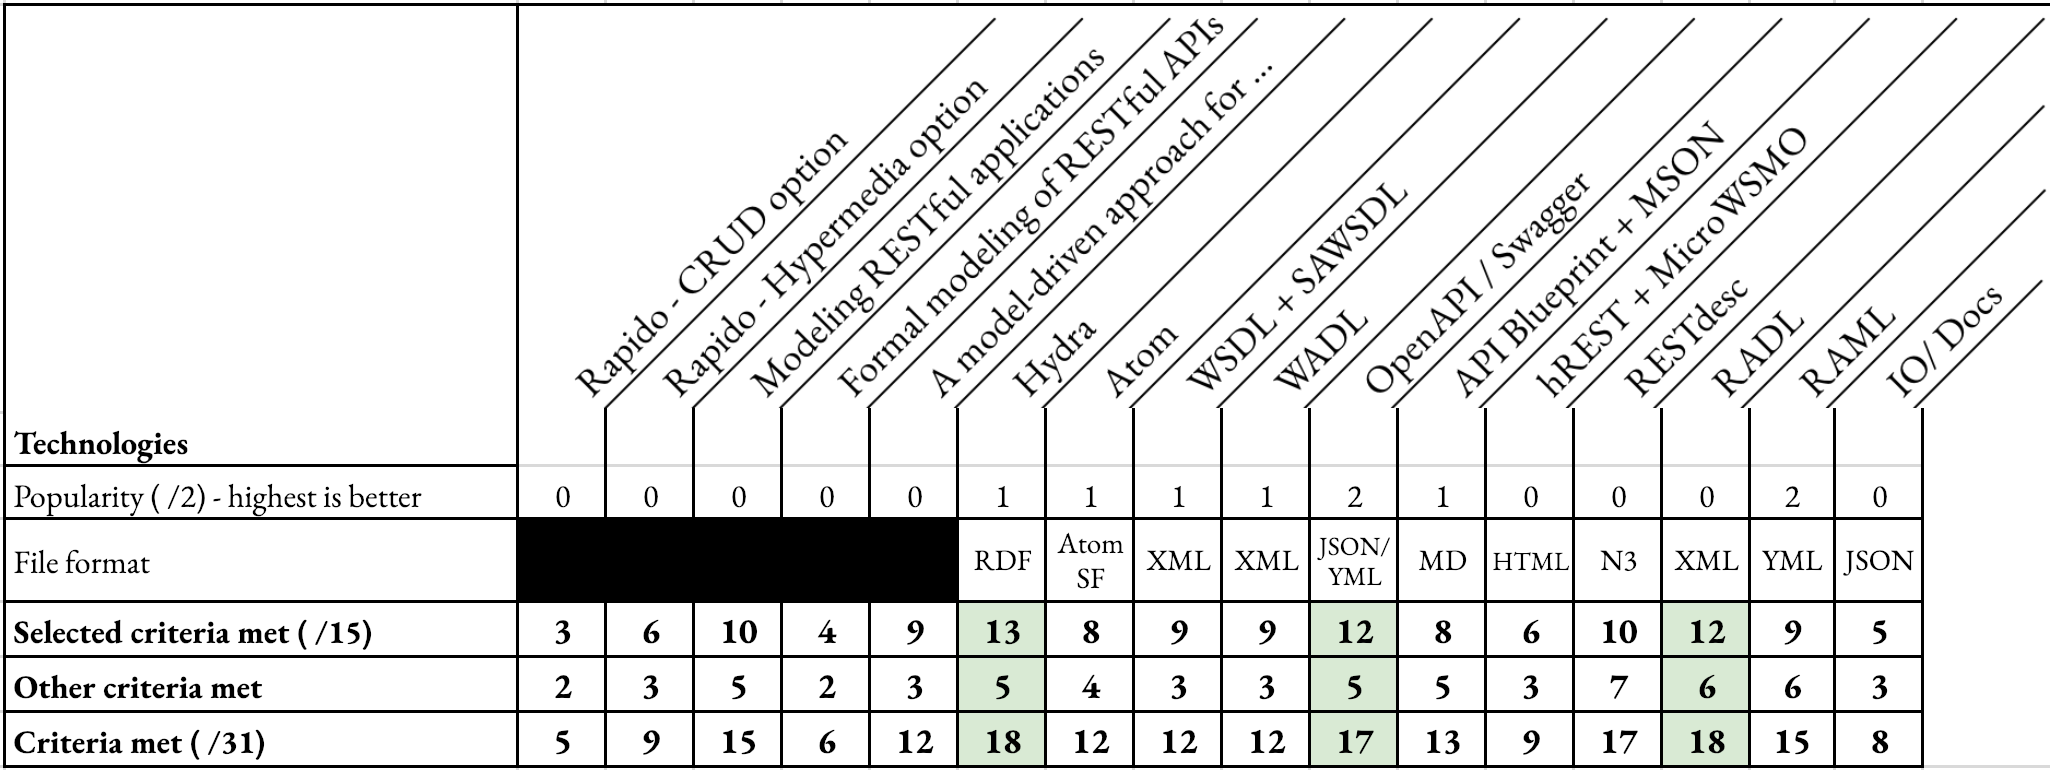
\includegraphics[width=0.8\textwidth]{figures/example-idl-results.png}
\label{example-idl-results}
\vspace*{-0.5cm}
\end{figure}

\begin{figure}[ht]
\caption{Results for data interchange formats}
\centering
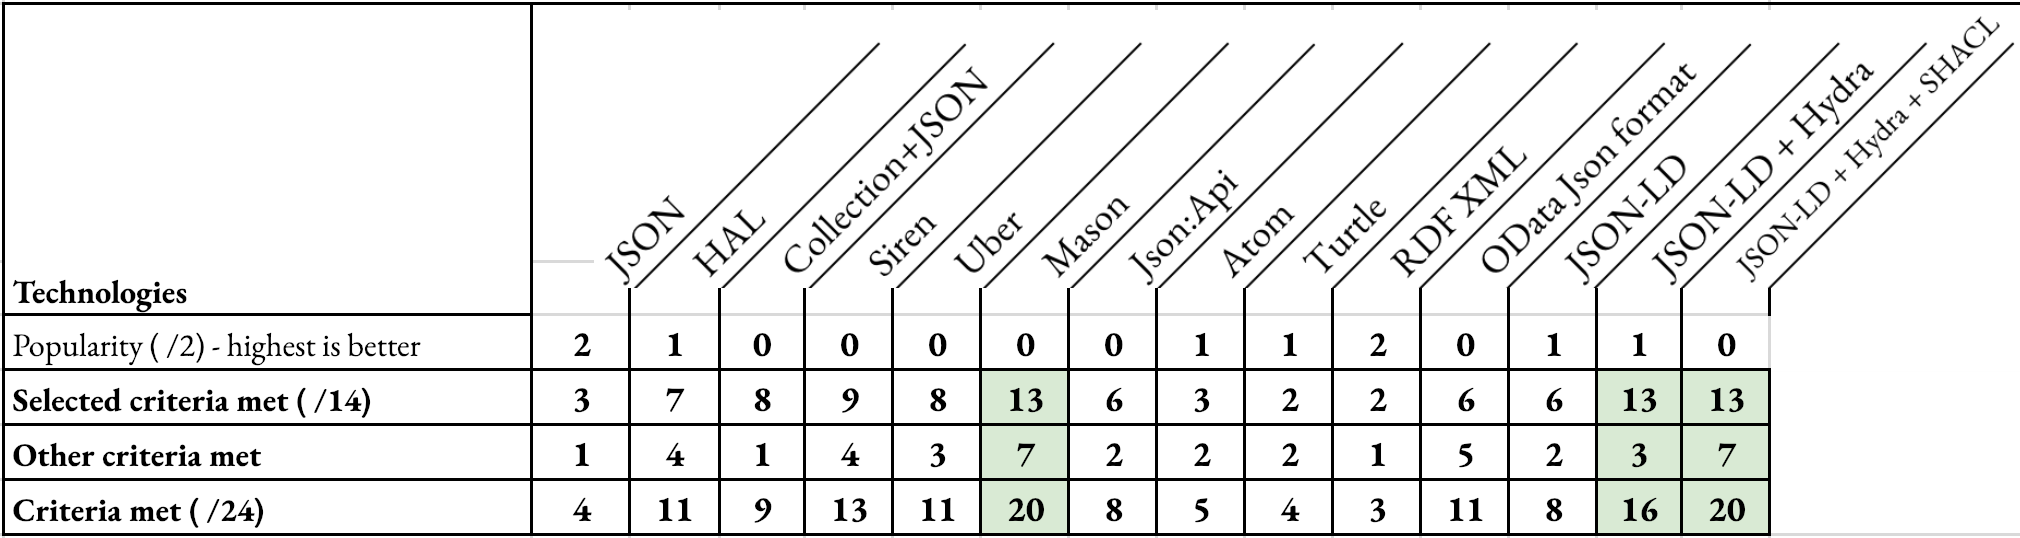
\includegraphics[width=0.8\textwidth]{figures/example-dif-results.png}
\label{example-dif-results}
\vspace*{-0.5cm}
\end{figure}

\begin{figure}[ht]
\caption{Results for implementation frameworks}
\centering
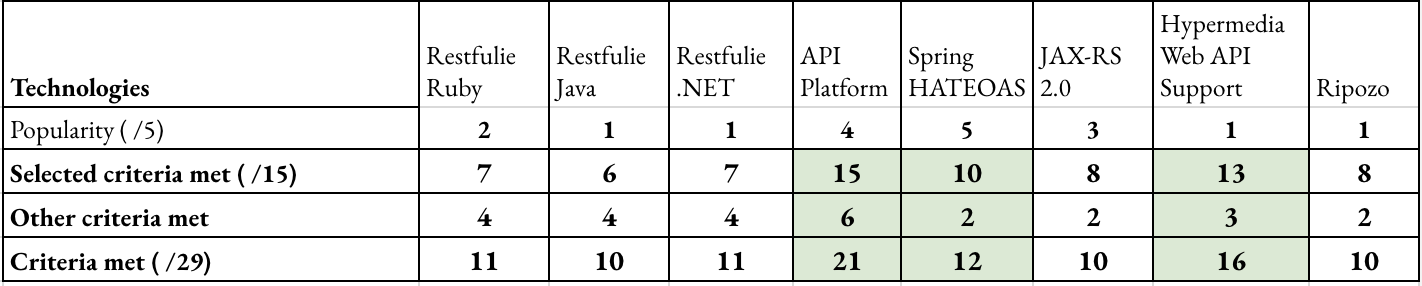
\includegraphics[width=0.8\textwidth]{figures/example-frameworks-results.png}
\label{example-frameworks-results}
\vspace*{-0.3cm}
\end{figure}

\paragraph{Interface Description Languages}
Hydra, OpenAPI and RADL are the technologies matching the highest number of selected criteria. However, none matches all criteria. Hydra lacks the ability to describe non-functional properties and media-types, which can be done with other RDF vocabularies. RADL lacks the ability to semantically describe resources models, operations, errors and non-functional properties, which can also be done with other vocabularies. On the other hand, OpenAPI does not support the usage of RDF vocabulary. 
In this project, we have chosen to setup both Hydra and OpenAPI. OpenAPI because it has most features and it is a must-have today because of its tooling and popularity. Hydra because it can be easily completed with other vocabularies and used with JSON-LD.

\paragraph{Interchange Formats}
Mason, JSON-LD + Hydra are the two technologies matching the highest number of selected criteria. JSON-LD + Hydra + SHACL is ignored as it does not match more selected criteria than without SHACL. While JSON-LD + Hydra lacks the ability to describe non-functional properties, Mason does not allow to use RDF vocabularies. Being incompatible with RDF requires a lot more effort to compensate than finding another vocabulary. This explains why JSON-LD + Hydra was preferred over Mason in this context.

\paragraph{Implementation frameworks}
API Platform, Spring HATEOAS and Hypermedia Web API Support \cite{salvadori2014framework} are the three technologies matching the highest number of criteria. The latter is immediately removed from the candidates because no public library is available. In this example, API Platform should be preferred over Spring HATEOAS because it matches five more criteria than Spring. However, developers of the companies we worked with know Java and not PHP. Moreover the Spring framework is very popular with them, which compensates the need to develop some features by hand. This is why we decided to go with Spring HATEOAS.

\paragraph{Easing the selection of the technologies}
We have developed an open-source web application{\footnote{\url{https://antoinecheron.github.io/morice/}}} in which the user selects the type of technology, the required criteria and finally \textit{score} each criterion to indicate its importance. 
In return, the web application presents the list of technologies that meet the required criteria ordered by their respective \textit{score}.
By offering a two-step wizard, we reduce the process of identifying relevant technologies to a few minutes.

% We developed an open-sourced web wizard to ease the selection of the technologies. It is accessible online\footnote{\url{https://antoinecheron.github.io/morice/}}.

% This tool is intended to be improved in future works.